\chapter{Suboptimal strategies for P3}
\label{chap:p3-suboptimal}

In this section, we take a look at some strategies and use them for scheduling with three processors. We will do so very exemplarily and inspect counterexamples for the respective strategies.

\todo{Introductory text}

\section{HLF}
\label{sec:hlf-p3-suboptimal}

First of all, we take look at some examples that show that HLF is not optimal for the three processor case. We will consider several phenomena that can occur if we use HLF with three processors.

\subsection{HLF does not behave the same for intrees with same profile}
\label{sec:p3-suboptimal-hlf-same-profiles-different-run-times}

In the two-processor case it is known that trees with the same level profile (see section \ref{sec:p2-profiles}) have the same run time. This is not the case for three processors \todo{Erklären, warum der Beweis nicht mehr hinhaut!} Figure \ref{fig:hlf-001112} shows an intree, where HLF can choose at some points, and different choices result in different runtimes.

\begin{figure}[ht]
  \centering
  \begin{subfigure}{.45\linewidth}
    \centering
    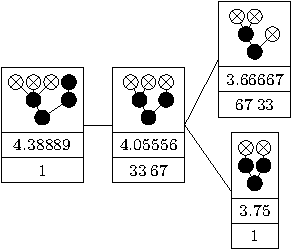
\includegraphics{p3/hlf_not_optimal/001112_hlf_subopt.pdf}
    \caption{Suboptimal HLF run}
  \end{subfigure}
  \begin{subfigure}{.45\linewidth}
    \centering
    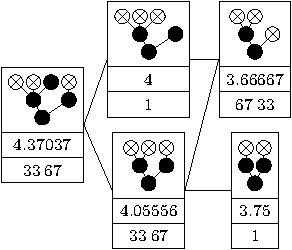
\includegraphics{p3/hlf_not_optimal/001112_hlf_opt.pdf}
    \caption{Optimal HLF run. This is also the overal optimal schedule.}
    \label{fig:hlf-001112-optimal-version}
  \end{subfigure}
  \caption{HLF on $(0,0,1,1,1,2)$. Different runs of HLF do not necessarily produce the same result.}
  \label{fig:hlf-001112}
\end{figure}

Because HLF can produce different run times depending which task it has chosen, it is clear that HLF in its raw form can not be optimal. The following section reveals even more.

\subsection{Examples where HLF is strictly suboptimal}
\label{sec:p3-suboptimal-hlf-strictly-suboptimal}

The example from figure \ref{fig:hlf-001112-optimal-version} shows the optimal run. We observe that this run is a specific instance of HLF, because at each point of time, always tasks with the highest level numbers are chosen.

However, there are intrees, where \emph{no} HLF-run is optimal. Figures \ref{fig:hlf-vs-opt-0012346688}, \ref{fig:hlf-vs-opt-0012446788} and \ref{fig:hlf-vs-opt-00123455799} show some examples for which this is exactly the case.

\begin{figure}[ht]
  \centering
  \begin{subfigure}{.45\linewidth}
    \centering
    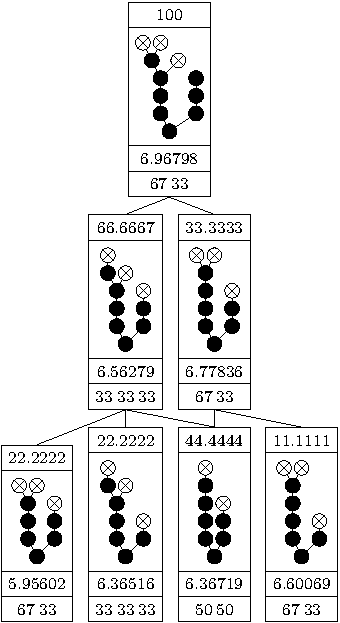
\includegraphics{p3/hlf_not_optimal/0012346688_subopt.pdf}
    \caption{HLF -- suboptimal}
  \end{subfigure}
  \begin{subfigure}{.45\linewidth}
    \centering
    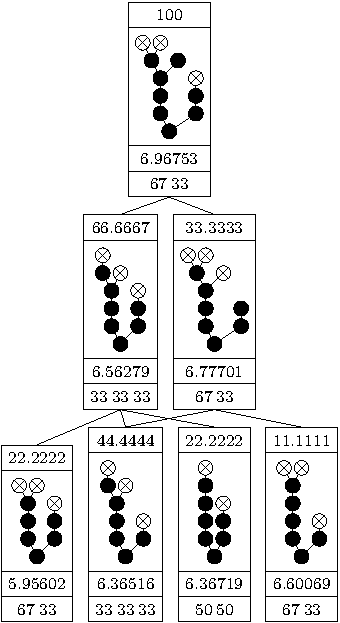
\includegraphics{p3/hlf_not_optimal/0012346688_opt.pdf}
    \caption{Optimal run is non-HLF}
  \end{subfigure}
  \caption{HLF vs. optimal solution for $(0,0,1,2,3,4,6,6,8,8)$}
  \label{fig:hlf-vs-opt-0012346688}
\end{figure}

\begin{figure}[ht]
  \centering
  \begin{subfigure}{.45\linewidth}
    \centering
    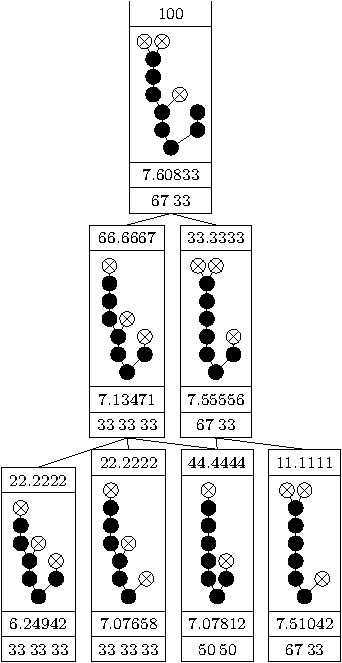
\includegraphics{p3/hlf_not_optimal/0012446788_subopt.pdf}
    \caption{HLF -- suboptimal}
  \end{subfigure}
  \begin{subfigure}{.45\linewidth}
    \centering
    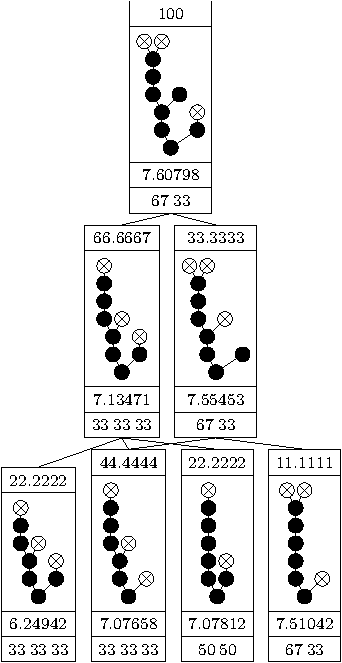
\includegraphics{p3/hlf_not_optimal/0012446788_opt.pdf}
    \caption{Optimal run is non-HLF}
  \end{subfigure}
  \caption{HLF vs. optimal solution for $(0,0,1,2,4,4,6,7,8,8)$ (taken from Ernst Mayr)}
  \label{fig:hlf-vs-opt-0012446788}
\end{figure}
\begin{figure}[ht]
  \centering
  \begin{subfigure}{.45\linewidth}
    \centering
    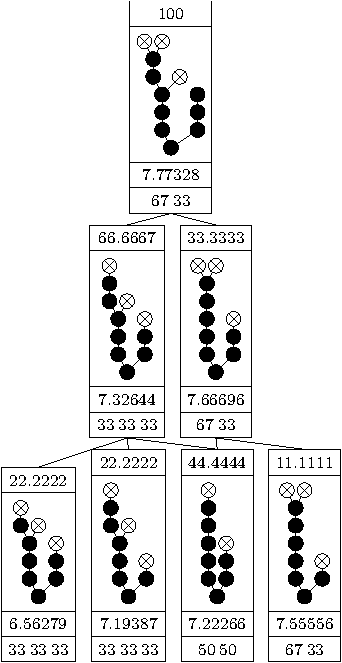
\includegraphics{p3/hlf_not_optimal/00123455799_subopt.pdf}
    \caption{HLF -- suboptimal}
  \end{subfigure}
  \begin{subfigure}{.45\linewidth}
    \centering
    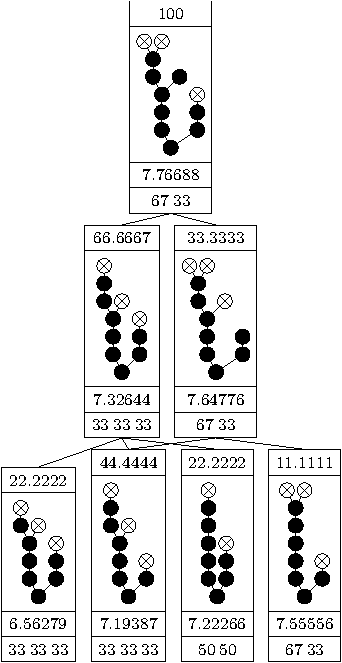
\includegraphics{p3/hlf_not_optimal/00123455799_opt.pdf}
    \caption{Optimal run is non-HLF}
  \end{subfigure}
  \caption{HLF vs. optimal solution for $(0,0,1,2,3,4,5,5,7,9,9)$ (taken from Chandy/Reynolds)}
  \label{fig:hlf-vs-opt-00123455799}
\end{figure}

\subsection{Different categories of sub-optimality}
\label{sec:hlf-suboptimal-two-variants}

As we saw, there are two possibilities for the sub-optimality of HLF:

\begin{itemize}
\item \emph{Not each possible run} of HLF yields the same run time.
\item The optimal run has to choose a strict non-HLF task.
\end{itemize}

We use the following nomenclature: A strategy is called \emph{can-optimal} (a term already used in \cite{MoritzMaasDiploma}), if it \emph{might} result in an optimal schedule. A strategy that \emph{can not} produce an optimal solution is called \emph{strictly suboptimal} (or simply suboptimmal if it is clear from the context). 

It is a notable fact that there are many cases, where HLF is can-optimal. For these cases, we examined several patterns and show -- for each of them -- an example where it is not optimal.

\section{Non-HLF strategies}
\label{sec:suboptimal-non-hlf-strategies}

We saw in the previos section that there are examples where HLF is strictly suboptimal. We now present some strategies that we took into consideration and that we examined w.r.t. their optimality. These strategies are strongly different from HLF and rely upon the structure of the intree. None of the strategies considered lead us to strictly optimal results in all cases.

\subsection{``2-HLF plus 1''}
\label{sec:disproving-2hlf-plus-1}

We examined all intrees with up to 13 tasks, especially the cases where HLF is not optimal. Thereby, we obsered that in all cases where three tasks could be scheduled, the optimal solution scheduled two tasks, that could be chosen by HLF for two processors and only the third task \emph{might} be a task that would not have been chosen by HLF (see figures \ref{fig:hlf-vs-opt-0012346688}, \ref{fig:hlf-vs-opt-0012446788} and \ref{fig:hlf-vs-opt-00123455799} as particular instances of those). Thus, we examined whether an optimal scheduling strategy for three processors has always \emph{at most one} task that is non-HLF. Interestingly, there is an intree with 15 tasks\todo{Eher den mit 14 Tasks reinhauen: $(0,0,1,2,2,3,3,6,8,9,10,11,12)$}, whose optimal schedule starts out by choosing the single topmost task and \emph{two} non-HLF tasks. This intree ($(0,0,1,2,2,3,3,6,8,9,10,11,12,13)$) is shown in figure \ref{fig:2-hlf-plus-one-not-optimal}. Another tree showing this fact is e.g. $(0, 0, 1, 2, 3, 4, 4, 5, 5, 8, 10, 11, 12)$.

\begin{figure}[ht]
  \centering
  \begin{subfigure}{.45\textwidth}
    \centering
    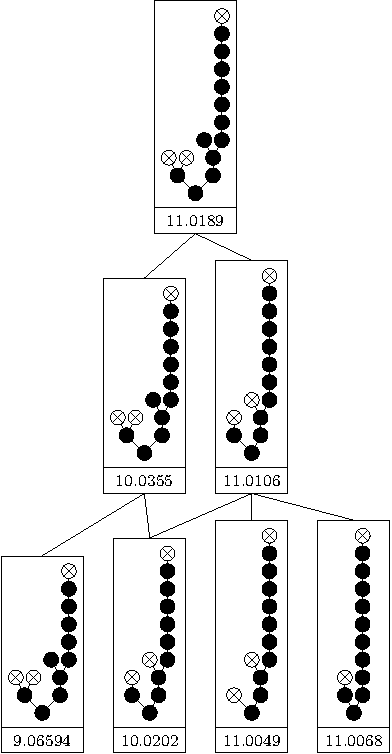
\includegraphics{p3/2hlf_suboptimal/001223368910111213_opt.pdf}
    \caption{Optimal schedule picking \emph{two} non-HLF tasks.}
  \end{subfigure}
  \quad
  \begin{subfigure}{.45\textwidth}
    \centering
    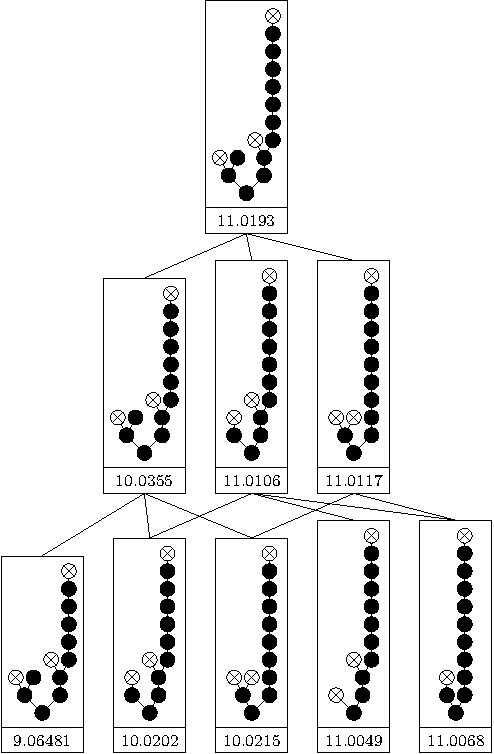
\includegraphics{p3/2hlf_suboptimal/001223368910111213_subopt.pdf}
    \caption{HLF-Schedule}
  \end{subfigure}
  \caption{Intree $(0,0,1,2,2,3,3,6,8,9,10,11,12,13)$ requires the optimal schedule to start out by choosing two non-HLF tasks.}
  \label{fig:2-hlf-plus-one-not-optimal}
\end{figure}

\subsection{``As few free paths as possible''}
\label{sec:disproving-hlf-no-free-chain}

(For now,) we call a path from the root to a leaf (i.e. a ready task) $t$ \emph{free} if $t$ is not scheduled.

One might be tempted to think that it should be the foremost goal to exploit parallelism as good as possible and that this might be acchieved by choosing the currently scheduled tasks in a manner such that as few free paths as possible in an optimal schedule. That is, we choose the leaves in a way so that the ends of as many different paths as possible are scheduled. This strategy was inspired by looking at the counterexamples against HLF depicted in figures \ref{fig:hlf-001112}, \ref{fig:hlf-vs-opt-0012346688}, \ref{fig:hlf-vs-opt-0012446788} and \ref{fig:hlf-vs-opt-00123455799}. We observe for these intrees that the optimal schedules has no as few free chains as possible.

However, there are examples where this strategy does not yield optimal results. Consider e.g. the tree $(0,0,0,1,1,1,2,2,3)$ (figure \ref{fig:hlfnfc-is-not-optimal} compares the optimal schedule to the no-free-paths schedule).

\begin{figure}[ht]
  \centering
  \begin{subfigure}{.45\textwidth}
    \centering
    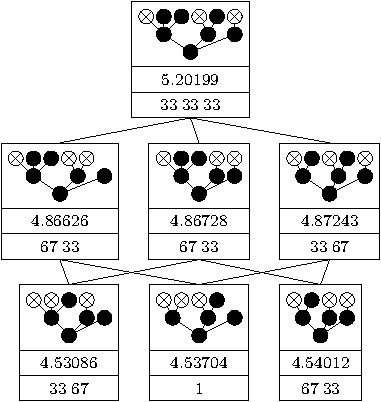
\includegraphics{p3/hlfnfc_not_optimal/000111223_hlfnfc.pdf}
    \caption{HLF schedule while choosing tasks such that there are as few free paths as possible -- overall run time of 5.20199.}
  \end{subfigure}
  \quad
  \begin{subfigure}{.45\textwidth}
    \centering
    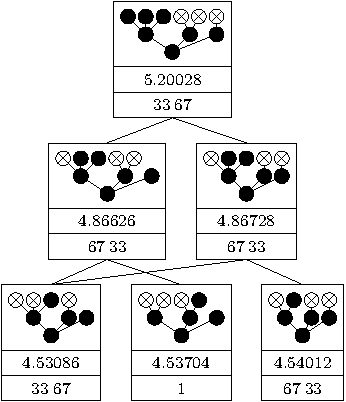
\includegraphics{p3/hlfnfc_not_optimal/000111223_opt.pdf}
    \caption{Optimal schedule (run time 5.20028) has three free paths at the beginning.}
  \end{subfigure}
  \caption{HLF with as few free paths as possible is not necessarily optimal.}
  \label{fig:hlfnfc-is-not-optimal}
\end{figure}

\subsection{Only highest or lowest leaves}
\label{sec:disproving-only-highest-or-lowest-leaves}

So far, we have seen several scenarios where HLF was not optimal. The trees we examined resulted in schedules that picked only combinations highest leaves and lowest leaves possible. Thus, we were tempted to think that an optimal schedule chooses only topmost tasks or leaves whose level is minimal (among all leaves). However, this is not a criterion for an optimal schedule, as we can observe by scheduling the 14-tasks-intree $(0,0,0,2,3,4,5,7,7,9,10,10,12)$, which is shown in figure \ref{fig:only-high-or-low-not-optimal}.

\begin{figure}[ht]
  \centering
  \begin{subfigure}{.45\textwidth}
    \centering
    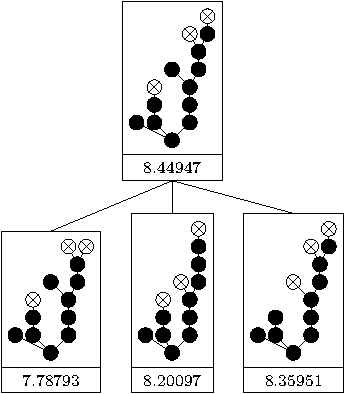
\includegraphics{p3/only_high_or_low/0002345779101012_opt.pdf}
    \caption{Optimal schedule picking a non-HLF task that is also not the lowest possible.}
  \end{subfigure}
  \quad
  \begin{subfigure}{.45\textwidth}
    \centering
    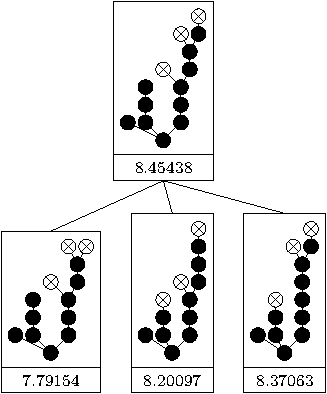
\includegraphics{p3/only_high_or_low/0002345779101012_subopt.pdf}
    \caption{Suboptimal HLF-Schedule.}
  \end{subfigure}
  \caption{Intree $(0,0,0,2,3,4,5,7,7,9,10,10,12)$ shows that there are intrees where an optimal schedule has to choose a non-HLF task that has a higher level than some non-chosen task.}
  \label{fig:only-high-or-low-not-optimal}
\end{figure}

\section{Special cases where HLF is can-optimal}
\label{sec:suboptimal-hlf-can-optimal-strategies}

As mentioned in section \ref{sec:hlf-suboptimal-two-variants}, there are many cases where HLF is \emph{can-optimal}, i.e. where the optimal schedule always has tasks of the highest levels scheduled, but not each HLF schedule is optimal. This results from situations where HLF can choose one from several task as the next task to be scheduled. We describe some strategies that try to eliminate these ambiguities and give counterexamples that show that these strategies are not optimal.

\subsection{Subtree with minimum number of topmost tasks}
\label{sec:suboptimal-hlf-can-optimal-subtree-fewest-toptasks}

If we consider the intree $(0,0,0,1,1,1,2,2,3)$, we have seen that an optimal schedule picks 7,8 and 9 as initially scheduled tasks (see figure \ref{fig:hlfnfc-is-not-optimal}). Moreover, in many cases, topmost-tasks that are the \emph{single direct predecessor} of their respective direct successor, are chosen by an optimal schedule.

These facts lead us to the suspicion that -- if we have an intree for which HLF is can-optimal -- (informally) we should pick the subtrees with the lowest number of topmost tasks. 

In this context, it is important to exactly describe which subtree we are talking about. Therefore, we employ the following definition:

\begin{definition}[Toptask-maximal subtree for a leaf]
  Let $t$ be a leaf of an intree $I$ and let $p=(t, t_1, t_2, t_3, \dots, r)$ be the path from $t$ to the root $r$.

  The \emph{toptask-maximal subtree for a leaf} $t$ is the subtree rooted at the \emph{lowest} task $t^*$ within $p$ that is not $t$ and that does \emph{not} contain more topmost tasks than the subtree rooted at the predecessor of $t^*$ within $p$.\todo{Versteht man das?}
\end{definition}

As an example, consider the following intree:

\begin{center}
  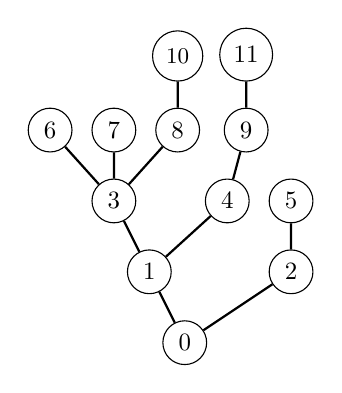
\begin{tikzpicture}[scale=.6, anchor=south]
    \node[circle, scale=0.9, draw] (tid0) at (3,1.5){0};
    \node[circle, scale=0.9, draw] (tid1) at (2.25,3){1};
    \node[circle, scale=0.9, draw] (tid2) at (1.5,4.5){3};
    \node[circle, scale=0.9, draw] (tid7) at (0.15,6){6};
    \node[circle, scale=0.9, draw] (tid10) at (1.5,6){7};
    \draw[ thick](tid2) -- (tid7);
    \draw[ thick](tid2) -- (tid10);
    \node[circle, scale=0.9, draw] (tid3) at (3.9,4.5){4};
    \node[circle, scale=0.9, draw] (tid5) at (2.85,6){8};
    \node[circle, scale=0.9, draw] (tid6) at (2.85,7.5){\small 10};
    \draw[ thick](tid5) -- (tid6);
    \draw[ thick](tid2) -- (tid5);
    \draw[ thick](tid1) -- (tid2);
    \draw[ thick](tid1) -- (tid3);
    \node[circle, scale=0.9, draw] (tid4) at (5.25,3){2};
    \node[circle, scale=0.9, draw] (tid9) at (4.3,6){9};
    \draw[ thick](tid3) -- (tid9);
    \node[circle, scale=0.9, draw] (tid11) at (4.3,7.5){11};
    \draw[ thick](tid11) -- (tid9);
    \node[circle, scale=0.9, draw] (tid8) at (5.25,4.5){5};
    \draw[ thick](tid4) -- (tid8);
    \draw[ thick](tid0) -- (tid1);
    \draw[ thick](tid0) -- (tid4);
  \end{tikzpicture}
\end{center}

The maximal subtree for leaf 10 is the subtree rooted at node 3, which can be derived as follows:
\begin{itemize}
\item The path from 10 to the root 0 is given by $p=(10,8,3,1,0)$.
\item We consider the subtrees rooted at the tasks along this path, and denote the subtree rooted at node $x$ by $I_x$:
  \begin{itemize}
  \item The subtree rooted at 10 (called $I_{10}$) contains only the topmost task 10.
  \item Subtree $I_8$ contains only topmost task 10.
  \item Subtree $I_3$ still contains only 10 as the topmost task (it introduces only a new leaf, namely 7).
  \item Subtree $I_1$ contains 10 \emph{and} 11 as topmost tasks.
  \end{itemize}
\item As seen, task 3 is the lowest task within $p$ that does not contain more topmost tasks than its predecessor.
\end{itemize}

A strategy for cases where HLF is can-optimal now might be to resolve HLF-ambiguities as follows:
\begin{itemize}
\item Generate all possible choices that could result from HLF.
\item For each topmost task, compute the topmost-maximal subtree.
\item Prefer topmost tasks whose topmost-maximal subtrees contain fewer topmost tasks.
\end{itemize}

The last step in the above explanation can be viewed as follows: We first create all possible choices of topmost tasks and then only choose those, whose

This strategy seems to do a good job in many cases, but can be seen to be false by examining the optimal schedule for the following intree with 18 tasks: $(0,0,1,1,2,3,3,4,5,7,8,9,9,11,13,13,13)$. It is shown in figure \ref{fig:subtree-with-fewest-toptasks-suboptimal}.

\emph{Remark:} We did not specify what should be done if there are several maximal subtrees with the same number of topmost tasks, but our counterexample suffices that this strategy does not work optimally even if there are no maximal subtrees with the same number of nodes.

\begin{figure}[ht]
  \centering
  \begin{subfigure}{.45\textwidth}
    \centering
    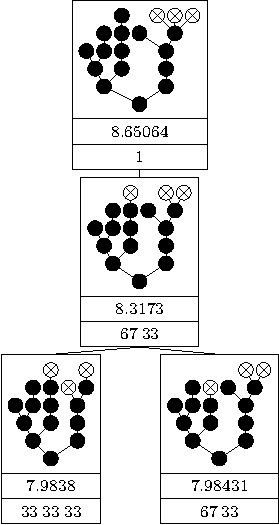
\includegraphics{p3/subtree_with_fewest_toptasks/subtree_with_fewest_toptasks_opt.pdf}
    \caption{Optimal schedule picking a subtree with three topmost tasks.}
  \end{subfigure}
  \quad
  \begin{subfigure}{.45\textwidth}
    \centering
    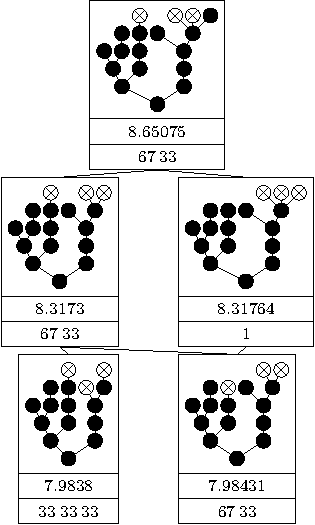
\includegraphics{p3/subtree_with_fewest_toptasks/subtree_with_fewest_toptasks_subopt.pdf}
    \caption{If we initially start with tasks as shown, this is the best schedule that can be obtained.}
  \end{subfigure}
  \caption{Intree $(0,0,1,1,2,3,3,4,5,7,8,9,9,11,13,13,13)$: For this intree, the optimal schedule chooses all tasks from a subtree with three topmost tasks and chooses none of the subtree with only one topmost tasks.}
  \label{fig:subtree-with-fewest-toptasks-suboptimal}
\end{figure}

\subsection{Subtree with maximum or minimum number of leaves}
\label{sec:suboptimal-hlf-can-optimal-subtree-fewest-leaves}

It can be quickly seen that slightly altering the strategy given in section \ref{sec:suboptimal-hlf-can-optimal-subtree-fewest-toptasks} in the sense that we do not concentrate on the number of \emph{topmost tasks} in a maximal subtree, but more generraly on the number of \emph{leaves} in a maximal subtree, does not yield a successful strategy. We adapt the notion of topmost-maximal subtrees in a straightforward manner:

\begin{definition}[Leaf-maximal subtree for a leaf]
  Let $t$ be a leaf of an intree $I$ and let $p=(t, t_1, t_2, t_3, \dots, r)$ be the path from $t$ to the root $r$.

  The \emph{leaf-maximal subtree for a leaf} $t$ is the subtree rooted at the \emph{lowest} task $t^*$ within $p$ that is not $t$ and that does \emph{not} contain more leaves than the predecessor of $t^*$ within $p$.
\end{definition}

\begin{description}
\item [Preferring leaf-maximal subtrees with fewer leaves] Figure \ref{fig:subtree-with-fewest-toptasks-suboptimal} shows that this strategy is not optimal, since the optimal solution prefers a subtree with four leaves over one with only three leaves.
\item [Preferring leaf-maximal subtrees with more leaves] One of our first examples, the intree $(0,0,0,1,1,1,2,2,3)$ (see figure \ref{fig:hlfnfc-is-not-optimal}) already shows that this strategy is not optimal in general.
\end{description}

\subsection{Prefer root's predecessors with longest processing time}
\label{sec:suboptimal-hlf-can-roots-longest-predecessors}

We also tried a recursive approach that decomposed an intree as follows: We separate the intrees rooted at the predecessors of the root. This way, we get a whole set of intrees. For each subtree, we now compute the optimal schedule and, moreover, the expected processing time -- assuming three processors in each individual subtree. The schedule for the whole intree then shall prefer subtrees whose expected processing time is the longest.

We were tempted to conjecture this because of the intree $(0,0,1,1,2,3,3,4,5,7,8,9,9,11,13,13,13)$ whose optimal schedule starts shown in figure \ref{fig:subtree-with-fewest-toptasks-suboptimal}. If we decompose this intree into its parts, we see that the subtree whose expected run time is maximal is the one whose tasks are initially scheduled in the optimal schedule (see figure \ref{fig:reasoning-for-longest-root-subtree}).

\begin{figure}[ht]
  \centering
  \begin{subfigure}{.45\textwidth}
    \centering
    \begin{tikzpicture}[scale=.2, anchor=south]
      \node[circle, scale=0.75, fill] (tid0) at (5.25,1.5){};
      \node[circle, scale=0.75, fill] (tid1) at (2.25,3){};
      \node[circle, scale=0.75, fill] (tid3) at (1.5,4.5){};
      \node[circle, scale=0.75, fill] (tid6) at (0.75,6){};
      \node[circle, scale=0.75, fill] (tid7) at (2.25,6){};
      \node[circle, scale=0.75, fill] (tid10) at (2.25,7.5){};
      \draw[](tid7) -- (tid10);
      \draw[](tid3) -- (tid6);
      \draw[](tid3) -- (tid7);
      \node[circle, scale=0.75, fill] (tid4) at (3.75,4.5){};
      \node[circle, scale=0.75, fill] (tid8) at (3.75,6){};
      \node[circle, scale=0.75, fill] (tid11) at (3.75,7.5){};
      \node[circle, scale=0.75, fill] (tid14) at (3.75,9){};
      \draw[](tid11) -- (tid14);
      \draw[](tid8) -- (tid11);
      \draw[](tid4) -- (tid8);
      \draw[](tid1) -- (tid3);
      \draw[](tid1) -- (tid4);
      \node[circle, scale=0.75, fill] (tid2) at (7.5,3){};
      \node[circle, scale=0.75, fill] (tid5) at (7.5,4.5){};
      \node[circle, scale=0.75, fill] (tid9) at (7.5,6){};
      \node[circle, scale=0.75, fill] (tid12) at (5.25,7.5){};
      \node[circle, scale=0.75, fill] (tid13) at (8.25,7.5){};
      \node[circle, scale=0.75, fill, task_scheduled] (tid15) at (6.75,9){};
      \node[circle, scale=0.75, fill, task_scheduled] (tid16) at (8.25,9){};
      \node[circle, scale=0.75, fill, task_scheduled] (tid17) at (9.75,9){};
      \draw[](tid13) -- (tid15);
      \draw[](tid13) -- (tid16);
      \draw[](tid13) -- (tid17);
      \draw[](tid9) -- (tid12);
      \draw[](tid9) -- (tid13);
      \draw[](tid5) -- (tid9);
      \draw[](tid2) -- (tid5);
      \draw[](tid0) -- (tid1);
      \draw[](tid0) -- (tid2);
    \end{tikzpicture}  
    \caption{Intree with initially scheduled tasks (for optimal schedule).}
  \end{subfigure}
  \quad
  \begin{subfigure}{.45\textwidth}
    \centering
    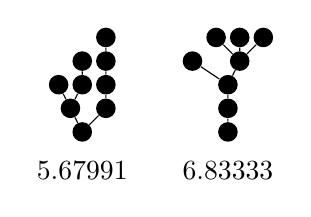
\begin{tikzpicture}[scale=.2, anchor=south]
      \node[circle, scale=0.75, fill] (tid1) at (2.25,3){};
      \node[circle, scale=0.75, fill] (tid3) at (1.5,4.5){};
      \node[circle, scale=0.75, fill] (tid6) at (0.75,6){};
      \node[circle, scale=0.75, fill] (tid7) at (2.25,6){};
      \node[circle, scale=0.75, fill] (tid10) at (2.25,7.5){};
      \draw[](tid7) -- (tid10);
      \draw[](tid3) -- (tid6);
      \draw[](tid3) -- (tid7);
      \node[circle, scale=0.75, fill] (tid4) at (3.75,4.5){};
      \node[circle, scale=0.75, fill] (tid8) at (3.75,6){};
      \node[circle, scale=0.75, fill] (tid11) at (3.75,7.5){};
      \node[circle, scale=0.75, fill] (tid14) at (3.75,9){};
      \draw[](tid11) -- (tid14);
      \draw[](tid8) -- (tid11);
      \draw[](tid4) -- (tid8);
      \draw[](tid1) -- (tid3);
      \draw[](tid1) -- (tid4);
      \node at (2.25, 0){5.67991};
      \begin{scope}[xshift=4cm]
        \node[circle, scale=0.75, fill] (tid2) at (7.5,3){};
        \node[circle, scale=0.75, fill] (tid5) at (7.5,4.5){};
        \node[circle, scale=0.75, fill] (tid9) at (7.5,6){};
        \node[circle, scale=0.75, fill] (tid12) at (5.25,7.5){};
        \node[circle, scale=0.75, fill] (tid13) at (8.25,7.5){};
        \node[circle, scale=0.75, fill] (tid15) at (6.75,9){};
        \node[circle, scale=0.75, fill] (tid16) at (8.25,9){};
        \node[circle, scale=0.75, fill] (tid17) at (9.75,9){};
        \draw[](tid13) -- (tid15);
        \draw[](tid13) -- (tid16);
        \draw[](tid13) -- (tid17);
        \draw[](tid9) -- (tid12);
        \draw[](tid9) -- (tid13);
        \draw[](tid5) -- (tid9);
        \draw[](tid2) -- (tid5);
        \node at (7.5, 0){6.83333};
      \end{scope}
    \end{tikzpicture}  
    \caption{Removing the root yields two subtrees with optimal expected runtimes (for three processors) as noted.}
  \end{subfigure}
  \caption{Intree $(0,0,1,1,2,3,3,4,5,7,8,9,9,11,13,13,13)$ and its corresponding subtrees rooted at the root's predecessors}
  \label{fig:reasoning-for-longest-root-subtree}
\end{figure}

Once again, this strategy can be shown to be suboptimal by considering $(0,0,0,1,1,1,2,2,3)$ (as depicted in figure \ref{fig:hlfnfc-is-not-optimal}) whose root has the following three predecessor intrees.

\begin{center}
  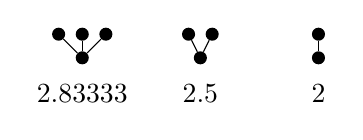
\begin{tikzpicture}[scale=.3]
    \begin{scope}
      \node[circle, fill, scale=.5] (0) at (0,0){};
      \node[circle, fill, scale=.5] (1) at (-1,1){};
      \node[circle, fill, scale=.5] (2) at (0,1){};
      \node[circle, fill, scale=.5] (3) at (1,1){};
      \draw(0)--(1);
      \draw(0)--(2);
      \draw(0)--(3);
      \node at (0, -1.5){2.83333};
    \end{scope}
    \begin{scope}[xshift=5cm]
      \node[circle, fill, scale=.5] (0) at (0,0){};
      \node[circle, fill, scale=.5] (1) at (-.5,1){};
      \node[circle, fill, scale=.5] (3) at (.5,1){};
      \draw(0)--(1);
      \draw(0)--(3);
      \node at (0, -1.5){2.5};
    \end{scope}
    \begin{scope}[xshift=10cm]
      \node[circle, fill, scale=.5] (0) at (0,0){};
      \node[circle, fill, scale=.5] (1) at (0,1){};
      \draw(0)--(1);
      \node at (0, -1.5){2};
    \end{scope}
  \end{tikzpicture}
\end{center}

\section{Maximizing 3-processor-time, minimizing 1-processor time}
\label{sec:p3-disproving-long-p3-and-short-p1-time}

Up to now, we maily focused on the structure of the current intree to derive strategies --- which all turned out to be (not strictly, but still) suboptimal. We now inspect another, more involved approach.

If we have three processors in total, we can split the total run time into three parts: The time where all three processors are processing tasks, the time where one processor is idle and two are working, and the time where only one processor is working.

%We first define some variants of run time. We consider the overall run time and the time where -- within a schedule of an intree -- exactly $p$ processors are working (i.e. where exactly $p$ tasks are scheduled).

\begin{definition}[Run time and its variants]
  We denote by $T$ the expected run time for a schedule associated with an intree. 
  Moreover, we denote the time where exactly $p$ taks are scheduled by $T_p$.
\end{definition}

Note that $T$ actually describes an \emph{expected value}. Because of the linearity of expectation, we have that -- for three processors -- $T=T_1 + T_2 + T_3$. If we want to construct an optimal schedule for three processors, we might be tempted to think that (at least) one of the two following criteria should be fulfilled for the optimal schedule:

\begin{description}
\item[P3L] For the optimal schedule, $T_3$ should be maximal (over all schedules), i.e. we should exploit three processors as long as possible (in the expectation).
\item[P1S] For the optimal schedule, $T_1$ should be minimal (over all schedules), i.e. we should try to keep the expected time for which only one processor is working as short as possible.
\end{description}

Surprisingly, \emph{both} of them are wrong (at least if considered separately).

\subsection{Maximizing $T_3$}
\label{sec:p3-disproving-long-p3}

Figure \ref{fig:p3-p3l-suboptimal-example} shows an example, where the optimal schedule keeps three processors busy for expected 0.77777 time steps, while a suboptimal schedule keeps three processors busy for a longer expected time, namely about 0.851852 time steps.

From this we can conclude that it may be advantageous in some cases to accept a shorter time with three busy processors, thereby possibly also decreasing the time where only one processor is busy.

\begin{figure}[ht]
  \centering
  \begin{subfigure}{.45\linewidth}
    \centering
    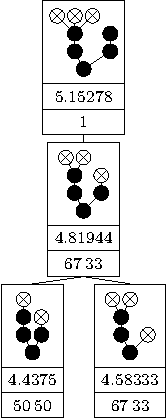
\includegraphics{p3/keep_3_busy/three_busy_opt.pdf}
    \caption{Optimal schedule. Keeps three processors busy for $7/9\approx 0.78$ time steps ($(T_3, T_2, T_1)=(7/9, 31/24, 37/12)$).}
  \end{subfigure}
  \quad
  \begin{subfigure}{.45\linewidth}
    \centering
    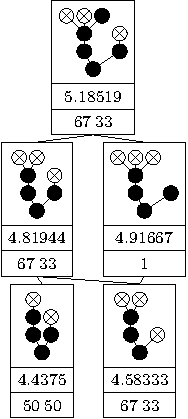
\includegraphics{p3/keep_3_busy/three_busy_subopt.pdf}
    \caption{This suboptimal schedule keeps three processors busy for expectedly $0.851852$ time steps ($(T_3, T_2, T_1)=(23/27,10/9,29/9)$).}
  \end{subfigure}
  \caption{An intree that shows that an optimal P3 schedule needs not keep busy three processors as long as possible. Snapshots with fewer than 6 tasks omitted since they have at most two tasks to be schedlued can be (optimally) processed via ordinary HLF. \todo{See figure \ref{fig:p3-p1s-suboptimal-example}!}}
  \label{fig:p3-p3l-suboptimal-example}
\end{figure}

\subsection{Minimizing $T_1$}
\label{sec:p3-disproving-short-p1}

The ``other direction'', i.e. minimizing the time where only one processor is busy, still is suboptimal.
Figure \ref{fig:p3-p1s-suboptimal-example} shows an intree with the property that the optimal schedule has an expected timespan of roughly 2.59259, within which only one processor is busy. On the other hand, a suboptimal schedule has a timespan of roughly 2.55555 within which only one processor is busy.

\begin{figure}[ht]
  \centering
  \begin{subfigure}{.45\linewidth}
    \centering
    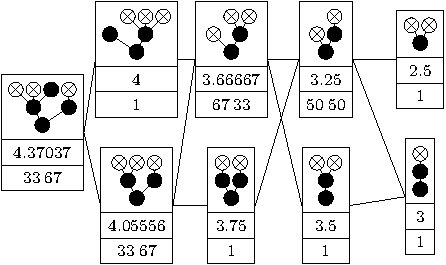
\includegraphics{p3/keep_1_unbusy/one_unbusy_opt.pdf}
    \caption{Optimal schedule. For expectedly $70/27\approx 2.59$ time steps, only one processor is busy $(T_3, T_2, T_1)=(23/27, 25/27, 70/27)$.}
  \end{subfigure}
  \quad
  \begin{subfigure}{.45\linewidth}
    \centering
    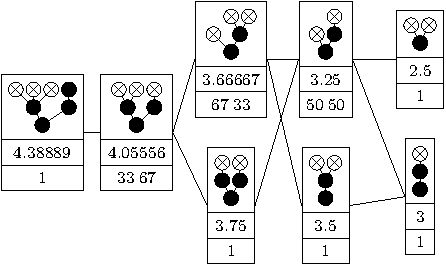
\includegraphics{p3/keep_1_unbusy/one_unbusy_subopt.pdf}
    \caption{This suboptimal schedule has an approximated timespan of $23/9\approx 2.55$ time steps, where only one processor is working ($(T_3, T_2, T_1)=(7/9,19/18,23/9)$).}
  \end{subfigure}
  \caption{An intree where the expected time with only one processor being busy is longer within the optimal schedule ($\approx 2.59259$) than within a suboptimal schedule ($\approx 2.555555$).}
  \label{fig:p3-p1s-suboptimal-example}
\end{figure}

This shows that it can be useful to accept a longer time with only one processor busy, probably acchieving a longer time span where three processors are busy.

\subsection{Maximizing $T_3$ \emph{or} minimizing $T_1$}
\label{sec:p3-suboptimality-maximizing-t3-and-minimizing-t1}

It can also be shown that even combining the two arguments -- in the sense that P3L \emph{or} P1S should be fulfilled for the optimal schedule -- is not correct. This can be observed by examining the intree $(0, 0, 1, 1, 2, 3, 3, 3)$. Figure \ref{fig:p3l-p1s-combo-suboptimal} shows this example.

\begin{figure}[ht]
  \centering
  \begin{subfigure}{.3\linewidth}
    \centering
    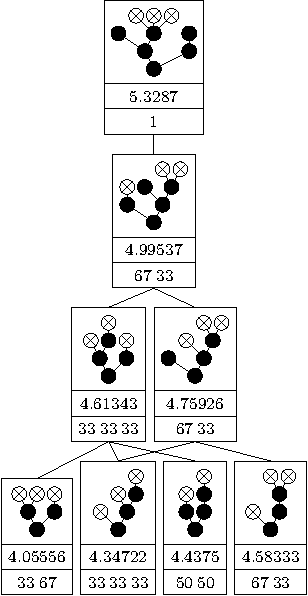
\includegraphics{p3/max_p3_min_p1/00112333opt.pdf}
    \caption{Optimal schedule. $(T_3^*,T_2^*,T_1^*)=(\frac{4}{3},\frac{217}{216},\frac{323}{108})$.}
  \end{subfigure}
  \quad
  \begin{subfigure}{.3\linewidth}
    \centering
    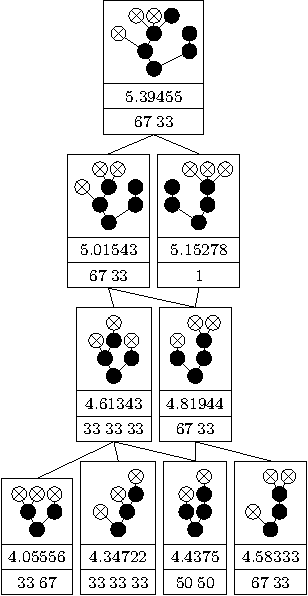
\includegraphics{p3/max_p3_min_p1/00112333t1min.pdf}
    \caption{Schedule with minimal $T_1$. $(T_3,T_2,T_1)=(\frac{290}{243},\frac{2369}{1944},\frac{2899}{972})$.}
  \end{subfigure}
  \quad
  \begin{subfigure}{.3\linewidth}
    \centering
    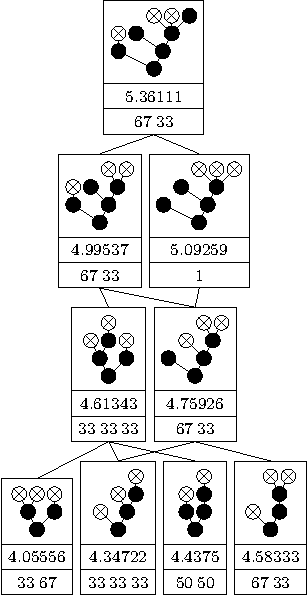
\includegraphics{p3/max_p3_min_p1/00112333t3max.pdf}
    \caption{Schedule with maximal $T_3$. $(T_3,T_2,T_1)=(\frac{110}{81},\frac{299}{324},\frac{499}{162})$.}
  \end{subfigure}
  \caption{A combination of P3L and P1S is not a criterion for an optimal schedule. The optimal schedule has $T_3^*=\frac{4}{3}\approx 1.333$ and $T_1^*=\frac{323}{108}\approx 2.99074$. One other (suboptimal) schedule has $T_1=\frac{2899}{972}\approx 2.98251 < T_1^*$, while still another schedule has $T_3=\frac{110}{81}\approx1.358025 > T_3^*$.}
  \label{fig:p3l-p1s-combo-suboptimal}
\end{figure}

\begin{corollary}
  Let $T^s$ denote the overall run time of a schedule $s$ and $T_1^s$, $T_2^s$ and $T_3^s$ be the times where exactly three, two and one tasks are scheduled within this schedule, respectively.

  Let $I$ be an intree and $S$ be the set of all schedules. Let $s^*$ be the optimal schedule, which has associated the optimal run time $T^*$, with $T_1^*, T_2^*, T_3^*$ being its parts.
  \begin{itemize}
  \item It may be the case that there is a schedule $s\in S$ such that $T_3^s \geq T_3^*$.
  \item It may be the case that there is a schedule $s\in S$ such that $T_1^s \leq T_1^*$.
  \end{itemize}
\end{corollary}

That is, it is not necessarily the case that $T_3$ is maximal for the optimal schedule, nor is it necessarily the case that $T_1$ is minimal for the optimal schedule.

However, after some investigation, we are tempted to conjecture the following.

\begin{conjecture}
  Let $I$, $T^s, T_1^s, T_2^s, T_3^s$ and $S$ be as defined above. Let $s^*$ be the optimal schedule for $I$ associated with the respective times $T_1^*, T_2^*, T_3^*$. Then, there is no schedule $s\in S$ such that
  \begin{equation*}
    T^s > T^* \wedge T_1^s \leq T_1^* \wedge T_3^s \geq T_3^*.
  \end{equation*}
\end{conjecture}

Even if this conjecture turns out to be true, it seems complex to transform this knowledge into a scheduling strategy that does something more significantly efficient than ``explore everything, and choose the best'', because $T_3, T_2$ and $T_1$ are not that easy to compute.

\section{Conclusion}
\label{sec:p3-conclusion}

Unfortunately, we did not find any strategy that always yields an optimal schedule. Of course, it is still possible to compute the optimal schedule by an exhaustive search.

During our research, we recognized some patterns that we are tempted to transform into some conjectures. We were, however, not yet able to prove or disprove them. This section shows the most important ones that could easily be used to decrease the number of snapshots that have to be examined if we want to compute the optimal snapshot by exhaustive search.

% \begin{definition}[Topmost task]
%   We say that a task is \emph{topmost} if its level is greater or equal than the levels of any other task in the intree. 
% \end{definition}

% \begin{conjecture}[Very likely]
%   For each snapshot resulting from an optimal schedule, at least one top-most task is scheduled.
% \end{conjecture}

% \begin{conjecture}[Weak one]
%   For each snapshot resulting from an optimal schedule, at least two top-most tasks are scheduled -- if there are two or more topmost tasks.
% \end{conjecture}

\begin{conjecture}
  An optimal schedule always schedules as many topmost tasks as possible.
\end{conjecture}

Please note that the above conjecture does not state anything about \emph{which} topmost tasks should be chosen in order to generate a schedule that is as good as possible.

\begin{conjecture}
  If for an intree only non-top tasks are scheduled, you can schedule any top-task instead of one non-top scheduled task to obtain a better run time.
\end{conjecture}

The main problems we faced when we tried to prove the above conjectures can be summarized as follows:
\begin{itemize}
\item The particular intree structure is not necessarily maintained over the induction step --- and if so, many case distinctions may be required.
\item Comparing different intrees seems to be quite cumbersome, especially if we do not know which tasks are scheduled.
\end{itemize}


%%% Local Variables:
%%% TeX-master: "../thesis.tex"
%%% End: 